\documentclass[./main.tex]{subfiles}

\begin{document}

\chapter{Introduction}\label{chapter:introduction}

"Only what is evolving is alive" \footnote{Pierre Kerner translation from french, original quote "N'est vivant que ce qui évolue"} -- this definition of life, like many others, is incomplete. And one could probably even find some counter-examples to it. One should first need to define what evolution is. We can try to define the evolution of a thing as its changes to optimize the capability to conserve itself. To do that, such a thing needs some form of memory.

In the majority of current known life, the physical support of this memory is DNA, which stands for DeoxyriboNucleic Acid. DNA is a molecule composed of two strands. Each strand is composed of a phosphate backbone. Along these backbones, we have a sugar linked to a nucleic acid. We have four types of nucleic acids: Adenine (A), Thymine (T), Cytosine (C) and Guanine (G), Figure \ref{intro:fig:dna_rna_pres} shows the 3D structure of DNA.

The two strands of DNA are linked by their nucleic acids, with some rules. In front of an A we will always have a T, in front of a C we will always have a G and vice-versa. A DNA strand is thus the complementary of the other. %But we cannot add a new DNA base to each DNA strain at the same end, due to some of chemical properties that we will not detail here.  % pas compris donc supprimé (Rayan)
We say DNA is composed of two anti-parallel strands. By convention we will always represent DNA in one orientation and will omit the other.

In bioinformatics, we generally represent a DNA strand by a single string on a four letter alphabet (A, C, T, G). The properties described above allow us to reconstruct the composition of one strand from the other by using the complementary letters (replace A by T, T by A, C by G and G by C) and reverse the order.%AL %JSV

\begin{figure}[ht]
    \centering
    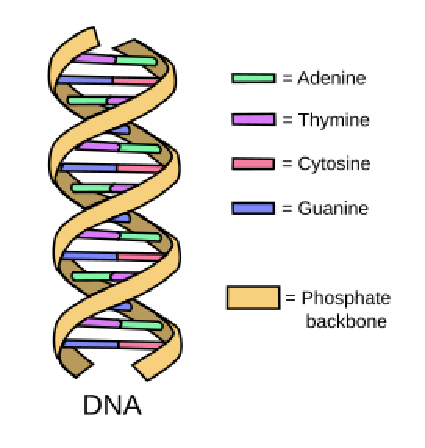
\includegraphics[width=5cm]{introduction/images/DNA.pdf}
    \caption{Structure and composition of DNA. Source: Wikipedia \protect\url{https://en.wikipedia.org/wiki/File:DNA_simple2.svg}}
    \label{intro:fig:dna_rna_pres}
\end{figure}

With many complex mechanisms, not detailed here, information contained in DNA is used to build essential molecules to keep the organism alive, and to reproduce it. %AL
This information is therefore the basis of the organism's functioning. If this information is destroyed or modified, the living organism will behave differently or die. Thus, knowing and understanding the succession of DNA bases is an effective entry point for analyzing many biological phenomena, diseases, and evolution. % JSV

To read this information, we rely on many biochemical techniques that we group under the term sequencing techniques. These techniques allow to read fractions of DNA fragments that are more or less long, and with various error rates. %AL %JSV

\section{Sequencing} \label{section:introduction:sequencing}

Sequencing technologies evolved quickly since 1977~\cite{sanger_sequencing}. Today we distinguish three generations of sequencing technologies, based on their properties.
In this section we focus on sequencing technologies properties and their impact on different bioinformatics tasks and do not detail the underlying biochemical methods.%AL

The two most important properties of a sequencing technology are the size of the DNA fragments it can read, expressed in number of bases, and also the number of errors that the technology will produce, expressed in percentage. An error rate of 0.1\% indicates that the sequencer will make one error every thousand bases.
When sequencing can read large fragments we have more information about the original sequence, which facilitates downstream analysis.
If a read contains many errors (replace a letter by an other one, insert random letter(s) or skip one or more letters), using the information provided by sequencing may be impossible or would require additional operations to correct those errors. Those operations will sometimes be very expensive, in terms of computer time.

\begin{table}[ht]
    \centering
    \begin{tabular}{ll|rr|l}
Generation & Technology          & Read length (bd)                 & Error rate             & Source                          \\ \hline
First      & Sanger              & $\approx$ 2 kb                   & Low ($\approx$ 2\%)    & \cite{seq_assembly_demystified} \\
Second     & ABI/Solid           & 75                               & Low ($\approx$ 2\%)    & \cite{seq_assembly_demystified} \\
Second     & Illumina/Solexa     & 100–150                          & Low ($<$2\%)             & \cite{seq_assembly_demystified} \\
Second     & IonTorrent          & $\approx$ 200                    & Medium ($\approx$ 4\%) & \cite{seq_assembly_demystified} \\
Second     & Roche/454           & 400–600                          & Medium ($\approx$ 4\%) & \cite{seq_assembly_demystified} \\
Third      & Pacific Biosciences & $\approx$ 10 kb ($\max$ 100 kb)  & High ($\approx$ 18\%)  & \cite{seq_assembly_demystified} \cite{longread_dark_matter} \\
Third      & Oxford Nanopore     & $\approx$ 10 kb ($\max$ 1 mb)    & High ($\approx$ 12\%)  & \cite{longread_dark_matter} \cite{nanopore_read_accuracy} \\
    \end{tabular}
    \caption{This table presents length of reads and error rate of main sequencing technology. Pacific Biosciences and Oxford Nanopore evolve quickly and different papers may report diverse figures.
    .}
    \label{intro:tab:technology_property}
\end{table}

Sanger technique produces long reads with very small error rate, but with a very low throughput and a very expensive cost per base. %AL
Second generation appeared in the mid-2000s. It increased the throughput and reduced the cost per base, but reduced dramatically the length of the reads and increases the probability of error ($\approx$ 1\%). %by orders of magnitude
The most frequent error type for this technology is a substitution between two nucleotides, (i.e. sequencer reads \texttt{A} in place of a \texttt{T}). %AL
Third generation dates back to the early 2010s. It has greatly increased the size of the reads but also the error rate while maintaining a good throughput. %decent ?
Errors in third generation are mostly insertion or deletion, sequencer didn't read a part of sequence or introduce random base not present in original sequence. Table \ref{intro:tab:technology_property} presents read lengths and error rates of many sequencing technologies. %AL
We would like to emphasize that both second and third generation technologies are still used today, and sometimes both technologies are used for a single experiment, as we will discuss later about hybrid techniques. %JSV

With sequencing one can read all information contained in a genome. But, no matter the technology, we get lots of (short) unordered fragments. Genome assembly therefore designates the task of reconstructing the original sequence from this set of unordered fragments. %AL

\section{The genome assembly task} \label{intro:sec:analogy}

If you want study an organism, knowing the complete genome sequence is very useful for a lot of tasks, such as as finding 
genes of interest, or study the sequence variations across a population \ldots %AL
Yet, the best sequencing technologies still provide reads that are at least 2 orders of magnitudes shorter than genomes. To understand the assembly problem, we provide a useful analogy which, to the best of our knowledge, has never been formulated before.

Imagine a crazy copyist monk. He is copying a book but he randomly chooses where he starts to copy. And he only copies small fragments of text at a time.
The copyist monk makes errors, e.g. he would sometimes replace a symbol by another one, would skip a symbol, or would add a random symbol. We call these errors substitutions, deletions and insertions, respectively.
Now imagine that there are multiple such copyist monks.
They choose randomly where they begin to write. They can choose several times the same region of the book or never choose to copy a certain region.
We refer by "coverage" the number of times a given chunk of the original book is copied. Coverage may significantly differ across the genome's regions. %AL
In this analogy, the book is the genome of the organism we want to study, and the copyist monks are our sequencer. The fragments of text are reads, and the operation to rebuild the book is assembly.

The assembly task can be seen as an ordering problem. %AL 
We try to put the text fragments in the original book order, and merge common parts at the end. %AL
To carry out this ordering, we could randomly take a fragment of text, and search among all the others if there exists a fragment that begins with the end of the one we took. In other words, the prefix of the sought fragment corresponds to the suffix of the taken fragment. When we observe this phenomenon we say that the fragments overlap. This a key concept in assembly. Once we have found the best overlap (generally the longest) for a text fragment we can merge the two fragments into one and restart our search for a new fragment that overlaps with the one we just created. And so on until there are no more fragments. This presentation of how to perform assembly is very simple, and in fact it is what we will later refer to as the greedy algorithm. We will see more advanced assembly algorithms in chapter \ref{chapter:sota}.

%\section{Assembly glossary} 
\bigskip

The genome assembly community, like any other scientific community, has its own set of concepts. 
%
A \textbf{read} designates a fragment of DNA produced by sequencer.
%
An \textbf{overlap} occurs between two reads when the suffix of a read is similar to the prefix of another read. The length of the common part is called the length of overlap.
%
A \textbf{contig} designates a sequence of DNA produced by an assembly tool. The exact definition of what is a \textbf{contig} changes between each assembly tool. We can see in some publications the term \textbf{unitig}: we will not get into details here, but a common fact is that contigs are built from unitigs.
%
A \textbf{scaffold} designates an ordering of contigs. Most of the times we cannot reconstruct each chromosome into a single contig. We describe some reasons for this fragmentation later. With external information such as restriction maps, linked reads, or targeted sequencing, one can order contigs and determinate approximately the number of bases in the gaps between contigs. %AL
%
Figure \ref{intro:fig:assembly} gives a summary of how reads are processed to obtain an assembly.
\begin{figure}[ht]
	\centering
	\subfile{introduction/tikz/assembly_lexique.tex}
	\caption{Schematic of DNA assembly. Each horizontal line represents a read, grey boxes represents overlaps found between reads. These overlaps are used to build contigs and finally these contigs are ordered into a scraffold.}
    \label{intro:fig:assembly}
\end{figure}

\section{Thesis outline}


As stated above, latest sequencing technologies allow to sequence larger DNA fragments. One could think that the task of assembly becomes easier since we have to solve a puzzle with larger pieces. But this is not the case, as we will see in the following chapters. The main goal of this work is improve long-read genome assembly without creating a new assembly tool or modifying an existing one. The tools developed in this thesis can interface with existing long-read assembly tools or even with other bioinformatics analysis tools.

Chapter \ref{chapter:preassembly} addresses some of the key steps that are performed prior to assembly. %AL
The quality of the data provided to an assembler has a direct impact on the produced results. %AL
This chapter describes the state of the art of tools used to detect overlaps between DNA fragments. The first contribution is a discussion on how to compare such tools. 
The second contribution of the chapter is a paper that presents two tools we developed during this thesis~\cite{yacrd}.
\yacrd  detects and removes regions with very high error rates in reads.
Experiments show that removing  low quality regions from reads improve assembly tools results. %AL
\fpa filters out uninformative overlaps in order to save disk space.

Chapter \ref{chapter:sota} presents a state of the art of several assembly methods, both from a theoretical point of view, and how they work in practice. This chapter introduces key concepts used in the next chapter.

Chapter \ref{chapter:postassembly} concerns some steps that occur after assembly. The first contribution is a blog post that presents the difficulties of evaluating the results of certain assembly tools that do not correct reads (or even polish contigs). The second contribution presents a tool for analyzing and improving assembly results, \knot, that we developed during this thesis \cite{knot}.

Chapter \ref{chapter:other_contribution} will focus on various other scientific contributions: participation in the development of a graphical interface for genomic data analysis, participation in the contest is, and some work around 10X data.

\end{document}